\PassOptionsToPackage{expansion=false}{microtype}
\documentclass[sigconf,nonacm]{acmart}

\usepackage{array}
\usepackage{booktabs}
\usepackage{amsmath}
\usepackage{graphicx}
\usepackage{balance}
\graphicspath{{paper/figures/}{figures/}{./}}
\setlength{\emergencystretch}{3em}

\title{Which Eviction Policy Should an LLM Cache Use?
A Systematic Study of Seven Policies Across Workloads,
Capacities, and Encoders}

\author{Yash Kulkarni}
\affiliation{
  \institution{University of Michigan}
  \city{Ann Arbor}
  \state{Michigan}
  \country{USA}
}
\email{yashkulk@umich.edu}

\author{Shubham Harkare}
\affiliation{
  \institution{University of Michigan}
  \city{Ann Arbor}
  \state{Michigan}
  \country{USA}
}
\email{sharkare@umich.edu}

\author{Arvind Suresh Yogesh Babu}
\affiliation{
  \institution{University of Michigan}
  \city{Ann Arbor}
  \state{Michigan}
  \country{USA}
}
\email{savyo@umich.edu}

\keywords{semantic caching, LLM serving, cache eviction,
comparative evaluation, approximate nearest neighbor, HNSW,
LMSYS, LLM-as-judge, quality-adjusted hit rate}

\setcopyright{none}
\acmConference[CSE 584]{CSE 584: Advanced Database Systems, Course Project}{Winter 2026}{Ann Arbor, MI}
\acmISBN{}
\acmDOI{}
\acmPrice{}
\settopmatter{printacmref=false, printccs=false, printfolios=true}

\begin{document}
\begin{abstract}
Caching is one of the few mechanisms that reduces both the latency and the cost of Large Language Model (LLM) serving without touching the model, and the space of proposed cache management algorithms has grown quickly. Practitioners can choose among classical replacement policies (FIFO, LRU, LFU, ARC, GDSF) and a newer family of semantic policies that exploit the geometry of the embedding space. These proposals have rarely been compared against one another on the same workloads under the same measurement protocol, so it is unclear which policy a deployment should actually use; this paper provides that comparison. Using CLEVER, an evaluation harness that also benchmarks Approximate Nearest Neighbor (ANN) indexes and a cost-aware adaptive router, we run seven eviction policies across three workloads (LMSYS-Chat-1M, Quora Question Pairs, MOSS), three cache capacities, and two embedding encoders, with three seeds per cell, and we audit the semantic validity of the resulting cache hits with an LLM judge.

Our main finding is that the choice of eviction policy is close to irrelevant on real conversational serving traces, and that two other design decisions dominate it. No policy beats LFU by more than 0.05\,pp in any of the eighteen dataset, capacity, and encoder cells, a margin of a handful of queries out of ${\sim}70$K, and every policy gap shrinks monotonically with capacity, effectively vanishing at a 30\% cache. The convergence has a structural cause. Because a query that hits is served without being re-inserted, the cache self-deduplicates and retains the residue of mutually distant entries, so even the most redundant workload we tested yields a cache whose internal redundancy is orders of magnitude too sparse for a semantic policy to exploit. Consistent with this, ARC converges to LFU's decisions, GDSF reduces to LFU-with-aging, and SISO, a policy designed specifically for LLM serving, performs at the level of a FIFO control on the sparse workloads (mean difference 0.096\,pp, and measurably worse than FIFO in nine of the twelve sparse-workload cells) while costing 3.1--3.5$\times$ LRU's per-query time. FIFO itself never beats LRU, which contradicts a contemporaneous report on agent memory buffers and locates the disagreement in the locality structure of the request stream. The first decision that does matter is calibration: hit thresholds do not transfer across encoders, and reusing one encoder's threshold under another silently produces a perfect measured hit rate that means nothing. The second is admission quality. An LLM judge, validated against an independently hosted judge ($\kappa = 0.826$), finds that most hits at the standard threshold are not semantically equivalent queries, collapsing quality-adjusted hit rates from 51--60\% to 1.1--2.2\% on LMSYS and QQP and from 98\% to 25\% on MOSS, and erasing the residual differences between policies into binomial noise. We conclude with concrete guidance: use LFU, spend the engineering effort on per-encoder threshold calibration and hit-quality auditing, and reserve semantically informed eviction for workloads whose cache-content redundancy has been measured and found dense.
\end{abstract}
\maketitle

\section{Introduction}
As Large Language Models (LLMs) scale in parameter count and context windows, the inference cost and latency bottleneck becomes a critical challenge for production systems \cite{kwon2023pagedattention}. Semantic caching mitigates this by intercepting queries before they reach the LLM, encoding them into a vector space, and performing a similarity search against previously answered queries. If a match is found within a defined distance threshold, the cached response is served, entirely bypassing the LLM.

A complete semantic caching system requires three pillars:
\begin{enumerate}
\item \textbf{Indexing:} Efficiently storing and retrieving high-dimensional vectors.
\item \textbf{Routing (Thresholding):} Deciding the distance threshold at which a cached response is a valid substitute for a fresh LLM call.
\item \textbf{Eviction:} Deciding which entries to remove when the cache reaches capacity.
\end{enumerate}

Of these three, eviction has attracted the widest range of competing proposals. Production systems such as GPTCache \cite{bang2023gptcache} default to classical heuristics like Least Recently Used (LRU) or Least Frequently Used (LFU), which were designed for exact-match keys and ignore the spatial relationships between embeddings. A second family argues that a semantic cache should instead optimize for semantic coverage: if two cached entries are highly similar they are mutually redundant, so evicting one costs little, while an isolated entry provides unique coverage and should be protected. Policies in this family include SISO \cite{kim2025siso}, designed specifically for LLM serving, the bandit formulation of Liu et al.\ \cite{liu2026semantic}, learning-augmented replacement for agent retrieval buffers \cite{sun2026solar}, and semantic-aware eviction for prefix caches \cite{fang2026prefix}. Between the two families sit hybrids from the classical literature, notably ARC \cite{megiddo2003arc} and GDSF \cite{cherkasova1998gdsf}, which combine recency and frequency signals adaptively.

Each of these policies has been evaluated in the setting its authors chose, on different corpora, at different cache capacities, under different embedding models, and against different baselines. A practitioner deciding what to deploy therefore has no basis for comparison, and the published claims sometimes point in opposite directions. Sun et al.\ \cite{sun2026solar}, for instance, report that LRU and LFU consistently lose to a naive FIFO baseline on semantic workloads, whereas in our measurements FIFO fails to beat LRU in any of eighteen cells and LFU leads throughout. Resolving disagreements of this kind requires running the policies against each other rather than reading across papers.

This paper provides that head-to-head comparison. We built CLEVER as a common harness so that every policy sees an identical query stream, an identical index, an identical similarity threshold, and an identical measurement protocol. We evaluate seven policies (FIFO, LRU, LFU, ARC, GDSF, SISO, and a semantic redundancy policy of our own design, included so that the semantic family is represented by an implementation we can instrument) across three workloads chosen to span the redundancy spectrum, three cache capacities, and two embedding encoders, with three seeds per cell. Because hit rate alone cannot distinguish a useful cache from a permissive one, we also audit the hits themselves with an LLM judge, and we report ANN index and router benchmarks that fix the rest of the serving path.

The comparison yields a clear and somewhat deflationary answer. Policy choice barely matters. No policy beats LFU by more than 0.05\,pp anywhere in the matrix, and all gaps shrink monotonically toward zero as capacity grows. The reason is structural rather than particular to any workload. A query that hits is served without re-insertion, so the cache continuously deduplicates itself and retains a residue of mutually distant entries, starving any policy that reasons about redundancy of the signal it needs. Two decisions that receive far less attention turn out to dominate the one that receives the most. Similarity thresholds do not transfer across encoders, and an uncalibrated threshold can produce a perfect measured hit rate while the cache serves arbitrary responses. Admission quality dominates even that: most hits at the standard threshold are not semantically equivalent queries, so the hit rates the policies compete over overstate delivered value by more than an order of magnitude.

\textbf{Contributions.} This paper makes the following contributions:
\begin{enumerate}
\item \textbf{A Controlled Seven-Policy Comparison:} The first head-to-head evaluation, to our knowledge, of FIFO, LRU, LFU, ARC, GDSF, SISO, and a semantic redundancy policy on a common harness, spanning three workloads, three cache capacities, two embedding encoders, and three seeds per cell. No policy beats LFU by more than 0.05\,pp in any cell, and every gap shrinks monotonically with capacity.
\item \textbf{A Mechanism for the Convergence:} A characterization of cache-content density showing that the admission rule deduplicates the cache against itself. The most redundant workload we tested (QQP) produces the sparsest cache contents, $20\times$ below LMSYS, because hits are never inserted. This explains why the convergence is structural rather than a property of any one corpus, and it predicts which workloads could escape it.
\item \textbf{Per-Encoder Threshold Calibration:} Evidence that similarity thresholds do not transfer across embedding encoders. Reusing a MiniLM-calibrated threshold under gte-base produces a degenerate cache with a 100\% measured hit rate, zero evictions, and no meaningful behavior at all. After recalibration the policy ordering replicates, but absolute hit rates differ by up to 19\,pp and not even consistently in direction.
\item \textbf{Quality-Adjusted Hit Rate:} An LLM-judged audit, cross-validated against an independently hosted judge ($\kappa = 0.826$ over 1{,}931 overlapping pairs), showing that most hits at the standard threshold are not semantically equivalent queries. Quality-adjusted hit rates collapse from 51--60\% to 1.1--2.2\% on LMSYS and QQP, policy differences fall within binomial noise, and near-zero embedding distance does not imply equivalence on templated prompts.
\item \textbf{Deployment Guidance:} A decision procedure (Section~\ref{sec:guidance}) tying the measurements to the choices a practitioner actually faces, including when the classical default suffices, what to measure before adopting a semantic policy, and which cost the policy will impose if adopted anyway.
\item \textbf{Serving-Path Benchmarks:} A comparison of FAISS index structures (Flat, HNSW, IVF, LSH) on 499K vectors establishing HNSW as Pareto-optimal (Recall@1 $= 0.989$ at $P50 = 0.52$ ms, a $34\times$ speedup over exact search for a 1.1\,pp recall loss), and a cost-based adaptive router achieving 60.33\% mean latency savings across five seeds.
\end{enumerate}

\section{Related Work}
\subsection{Semantic Caching for LLMs}
Semantic caching has emerged as a practical cost-reduction technique for LLM serving. GPTCache \cite{bang2023gptcache} provides a modular open-source architecture for embedding queries and searching them with vector backends such as FAISS \cite{johnson2019faiss}, relying on static similarity thresholds and classic eviction algorithms (LRU/LFU). Later systems extend this design along other axes: MeanCache \cite{gill2025meancache} moves the cache client-side for privacy, SCALM \cite{li2024scalm} clusters chat queries to identify cache-worthy entries, ContextCache \cite{yan2025contextcache} conditions matching on multi-turn context, and vCache \cite{schroeder2025vcache} replaces the global similarity threshold with per-entry learned thresholds that carry an error-rate guarantee. Liu et al.\ \cite{liu2026semantic} formalize semantic cache eviction as a Combinatorial Multi-Armed Bandit (CMAB) problem, balancing mismatch costs and serving costs online without prior knowledge of query distributions. Each of these systems must choose an eviction policy, but none compares candidate policies under a common protocol; that comparison is the subject of this paper.

\subsection{ANN Indexing and Vector Search}
Efficient similarity search over high-dimensional embeddings is a prerequisite for semantic caching at scale. FAISS \cite{johnson2019faiss} provides a widely adopted suite of ANN index structures. HNSW \cite{malkov2018hnsw} achieves state-of-the-art recall-latency tradeoffs through hierarchical graph navigation, making it the index of choice for low-latency retrieval. LSH \cite{indyk1998ann} offers sublinear search via random projections but degrades significantly under continuous $L_2$ distance thresholds, as our benchmarks confirm. Product Quantization \cite{jegou2011pq} enables memory-efficient approximate search by compressing embedding vectors into compact codes, which suits large-scale cache deployments where memory footprint is constrained.

\subsection{Cache Eviction Policies}
Classical eviction research provides the theoretical and practical foundation for our work. Belady's algorithm \cite{belady1966study} defines the optimal offline eviction policy by always evicting the entry whose next access is furthest in the future, serving as an unreachable theoretical upper bound for any online policy. LRU-K \cite{oneil1993lruk} extends recency-based eviction by tracking the K-th most recent access, improving robustness to sequential scan patterns that confound standard LRU. ARC \cite{megiddo2003arc} dynamically balances recency and frequency via two adaptive LRU lists, achieving strong performance without manual parameter tuning. All three operate on exact-match cache keys and are unaware of the continuous semantic space of LLM embeddings; the semantic policy family proposes to close this gap, which is why our comparison includes one such policy.

\subsection{Comparative Evaluations and Contemporaneous Work}
Several recent papers evaluate multiple replacement policies on semantic
workloads, and the picture they collectively paint is inconsistent, which is
part of what motivates a controlled comparison. Sun et al.\
\cite{sun2026solar} study eight policies on agent retrieval buffers and
report that LRU and LFU consistently underperform a naive FIFO baseline,
attributing this to absent temporal locality and frequency concentration in
their workloads. Our setting differs in what is being cached: they manage an
agent's stored experience over conversational memory benchmarks, whereas we
cache query-to-response pairs on serving traces of 100K queries and above.
On our workloads the ordering is the opposite, with FIFO last and frequency
information clearly useful at small capacities, which suggests that the
locality structure of the request stream, rather than the semantic matching
itself, determines whether classical signals retain value. We include FIFO
specifically so this comparison can be made directly (Section~\ref{sec:matrix}).

Fang et al.\ \cite{fang2026prefix} learn semantic-aware eviction for prefix
caches, operating on KV blocks inside the serving engine rather than on
completed query-response pairs; their reported reuse variation across token
types is a different phenomenon from the query-level redundancy we measure.
Baral et al.\ \cite{baral2026calibration} address threshold calibration in
semantic caching and argue that ranking metrics such as PR-AUC misrepresent
behavior at a fixed deployment threshold, proposing precision-at-cache-hit
metrics instead. Their work and ours reach a similar conclusion, that a
permissive threshold inflates apparent cache performance, from opposite
directions. They evaluate nine bi-encoders independently on a static labeled
sentence-pair benchmark, determine hit validity from ground-truth pair
labels, and study neither eviction nor the transfer of a calibrated
threshold from one encoder to another. We run a streaming cache simulation
in which admission and eviction interact, judge validity with an LLM on
hits the deployed threshold actually admitted, and show that transferring a
threshold across encoders fails outright. The two approaches are
complementary: their metrics describe how to choose a threshold, our
measurements describe what happens downstream when one is chosen badly. To our knowledge no prior study places the
classical policies, the LLM-serving-specific policies, and a semantic policy
on a single harness across workloads, capacities, and encoders, or pairs
that comparison with an audit of whether the measured hits are valid.

\subsection{Retrieval-Augmented Generation and Non-Parametric Memory}
Semantic caching is motivated by the broader success of retrieval-augmented generation (RAG) \cite{lewis2020rag}, which demonstrates that conditioning LLM outputs on retrieved context from non-parametric memory can substantially improve factual accuracy on knowledge-intensive tasks. This paradigm has been validated at scale: kNN-LM \cite{khandelwal2020knnlm} shows that retrieval over training corpora improves language model perplexity without additional training, RETRO \cite{borgeaud2022retro} demonstrates trillion-token retrieval gains in autoregressive generation, and Atlas \cite{izacard2023atlas} achieves competitive few-shot performance by tightly integrating retrieval with encoder-decoder models. Black-box approaches such as REPLUG \cite{shi2023replug} and adaptive self-reflective methods like Self-RAG \cite{asai2024selfrag} further demonstrate practical retrieval flexibility across deployment settings.

However, retrieval is not universally beneficial. Mallen et al.\ \cite{mallen2023trust} show that retrieval augmentation can actively hurt performance on facts well-memorized by parametric models, and Liu et al.\ \cite{liu2024lost} demonstrate that LLMs frequently fail to effectively utilize retrieved context positioned in the middle of long inputs. These results establish that the benefit of non-parametric retrieval is workload-dependent, a finding that directly motivates CLEVER's empirical approach to evaluating when semantic caching provides genuine value versus when simpler frequency-based policies dominate.

\section{System Architecture and Methodology}
CLEVER is organized as a sequence of modular components: an index benchmark, a cost-based router, an eviction layer hosting seven interchangeable policies, and an LLM-based audit of hit quality. This section describes each in turn.

\subsection{Index Benchmarking}
We wrap and evaluate four FAISS \cite{johnson2019faiss} index structures to determine the optimal backend for semantic caching:
\begin{itemize}
\item \textbf{Flat (Exact):} Exhaustive $L_2$ distance search, guaranteeing 1.0 recall.
\item \textbf{HNSW (Hierarchical Navigable Small World) \cite{malkov2018hnsw}:} A graph-based approach optimizing for rapid routing and high recall.
\item \textbf{IVF (Inverted File Index):} A partition-based approach optimizing for memory footprint and throughput via Voronoi cells.
\item \textbf{LSH (Locality-Sensitive Hashing):} Evaluated for extreme memory-constrained environments.
\end{itemize}

\subsection{Cost-Based Adaptive Router}
Static distance thresholds often fail to balance the cost of an LLM call against the degradation of response quality. We propose an adaptive router that learns an optimal $L_2^2$ distance threshold ($\theta$) from a calibration set. 

The router sweeps candidate thresholds to maximize a combined objective function:
\begin{equation}
\mathit{Obj} = \mathit{CostSavings}(\theta) - \lambda(1 - \mathit{Quality}(\theta))
\end{equation}
where $\mathit{CostSavings}$ is derived from a defined hardware cost
model, $\mathit{Quality}$ is proxied via cosine similarity
($1 - \frac{d^2}{2}$, where $d$ is the $L_2$ distance
between normalized vectors), and $\lambda = 2.0$ is a
penalty coefficient set to strongly suppress false cache
accepts, ensuring the router conservatively prefers cache
misses over low-quality hits. Embeddings are
$L_2$-normalized prior to indexing, making this
approximation exact.

\subsection{The Semantic Redundancy Policy}
The semantic policy in the comparison, from which CLEVER (Cluster-Level Eviction for Vector Embedding Retrieval) takes its name, scores entries by the ratio of their semantic redundancy to their historical utility.

\textbf{The Scoring Function:}
\begin{equation}
\mathit{score}(e) = \frac{r(e) + \mu}{\alpha \cdot \mathit{recency}(e) + \beta \cdot \mathit{frequency}(e) + \varepsilon}
\end{equation}

\begin{itemize}
\item \textbf{Redundancy $r(e)$:} The fraction of active cached entries within distance $\theta_e$ of $e$.
\item \textbf{$\mu$-Smoothing:} An additive Laplace-style constant. As $\mu \to \infty$, the semantic term is washed out, and the ordering approaches pure inverse-utility (LFU/LRU). This guarantees the policy degrades gracefully rather than failing entirely if the redundancy signal is absent.
\item \textbf{Recency Floor:} $recency(e)$ is ranked and floored at $1/N$. This prevents the oldest entry from driving the denominator to $\varepsilon$, which would cause its score to explode and render it ``immortal'' regardless of its redundancy.
\end{itemize}

\textbf{Incremental Symmetric Redundancy Graph:}
Computing $r(e)$ naively requires $O(N^2)$ distance calculations per eviction. We implement an incremental approach:
\begin{itemize}
\item \textbf{On Insert:} We sample $S \le 1024$ active entries, compute distances to the new entry $e$, and \textit{symmetrically} add edges to the neighbor graph for any pairs within $\theta_e$. This bounds insertion to $O(S)$.
\item \textbf{On Evict:} We remove the evicted node from the neighbor lists of its connected peers in $O(|neighbors|)$ time.
\item \textbf{Batch Rebuilds:} To correct for sampling bias, we perform periodic full rebuilds of the graph via FAISS batch search.
\end{itemize}

\subsection{Classical and LLM-Serving Policies}
A comparison restricted to LRU, LFU, and the semantic policy would be too narrow to support deployment guidance, so we add four further policies spanning arrival-order, adaptive, cost-aware, and LLM-cache-specific designs. Each must be adapted to a semantic cache, where entries are unit-norm embeddings and cache ids are slot-unique (an evicted id is never re-requested).

\textbf{FIFO} evicts the oldest insertion and ignores accesses entirely. It is the weakest policy that still functions as a cache, and it anchors the bottom of the comparison: any policy that fails to beat it is extracting no value from the recency, frequency, or geometric signals it consults. We include it also because Sun et al.\ \cite{sun2026solar} report it outperforming LRU and LFU on semantic workloads, a claim that cannot be checked against our matrix without running it.

\textbf{ARC} \cite{megiddo2003arc} balances a recency list $T_1$ against a frequency list $T_2$ using ghost lists $B_1$/$B_2$ of recently evicted keys; a request for a ghosted key adapts the target split $p$. Because our cache ids are slot-unique, a classic exact-match ghost hit can never fire. Our adaptation detects ghost hits semantically: each ghost retains the evicted entry's embedding, and an inserted query whose embedding lies within
$L_2^2 \le 0.20$ of a ghost (cosine ${\approx}\,0.90$ for unit-norm MiniLM vectors) counts as a ghost hit. This is the semantic-cache analogue of re-requesting a recently evicted item. On a match, $p$ adapts with the classic deltas, the ghost is retired, and the new entry is admitted directly to $T_2$; ghost lists are LRU-bounded at capacity $c$.

\textbf{GDSF} \cite{cherkasova1998gdsf} assigns each entry the priority $L + \mathit{frequency}(e) \cdot \mathit{cost}(e)/\mathit{size}(e)$, where the inflation clock $L$ rises to each victim's priority (aging). We instantiate $\mathit{cost}(e) = 1/\lVert e \rVert$ and $\mathit{size}(e)$ as the embedding dimension. On unit-norm, fixed-dimension embeddings every entry has $\mathit{cost} \approx 1$ and identical size, so the cost/size term is uniform and GDSF reduces to \emph{LFU-with-aging}; the general formula is implemented regardless.

\textbf{SISO} \cite{kim2025siso} is a recent (August 2025) caching policy designed specifically for LLM serving. Each cached entry acts as a cluster centroid carrying a \emph{cluster size} (semantic locality, long-term value) and an \emph{access count} (short-term popularity). On insert, the closest cached entry within the clustering threshold
$\theta_C = 0.86$ cosine ($L_2^2 < 0.28$) absorbs one unit of cluster mass; an insert that opens a new semantic region receives temporary infinite-access-count protection. Every 1{,}000 requests a maintenance round decays all cluster sizes by $1.1\times$ and resets access counts; eviction removes the entry with the lexicographically smallest (cluster size, access count) pair. SISO's original cache manager re-clusters query logs offline; our implementation maps its merge step to online per-insert merging with the search bounded at 1{,}024 sampled entries, and drives its M/D/1-based adaptive retrieval threshold $\theta_R$ from a sliding-window hit rate. As in the original design, $\theta_R$ does not influence victim selection. We therefore evaluate this adapted, online single-pass variant, denoted SISO throughout, rather than the original offline re-clustering manager; its results should be read as characterizing the streaming adaptation, and a comparison against the authors' reference implementation is left to future work.

All seven policies (FIFO, LRU, LFU, Semantic, ARC, GDSF, SISO) run under an identical harness: the policy only observes insert, access, and evict events and selects victims, while admission, lookup, the
$L_2^2 = 0.90$ hit threshold, and the 30\% warmup prefix are fixed by the cache. The judged hit-quality audit (Section~\ref{sec:judge}) predates the FIFO runs and therefore covers the other six policies only.

\subsection{Per-Encoder Threshold Calibration}
\label{sec:calibration}
Similarity thresholds are not portable across embedding models. Our MiniLM
configuration uses an $L_2^2$ hit threshold of $0.90$ (cosine $\geq 0.55$),
which sits at MiniLM's median nearest-neighbor cosine similarity ($0.553$)
over the 100K-query corpora. The second encoder, \texttt{gte-base} (768
dimensions) \cite{li2023gte}, is strongly anisotropic
\cite{ethayarajh2019contextual}: random query pairs
average cosine similarity $0.69$--$0.76$ across our three datasets, versus
approximately $0$ for MiniLM. A threshold of cosine $0.55$ therefore lies
below the random-pair mean under gte-base, and essentially every pair
of queries qualifies as a cache hit. A single universal threshold is thus
unsound; a threshold must occupy the same statistical position in each
encoder's similarity distribution.

We therefore recalibrate every distance-bearing parameter for gte-base by
anchoring it at the same quantile of the gte similarity distribution that the
MiniLM value occupies in MiniLM's. The hit threshold becomes $0.30$ $L_2^2$
(cosine $0.85$), the gte nearest-neighbor median; the semantic policy's
redundancy threshold moves with it ($0.30$, preserving the invariant that two
cached entries are neighbors if and only if one would be a hit for the other). SISO's
clustering and retrieval thresholds move from cosine $0.86$ to $0.94$
(the deep random-pair tail under both encoders), with its dynamic-threshold
floor raised from $0.60$ to $0.85$ so it cannot wander below gte's random-pair
mean ($\approx 0.74$). ARC's ghost-list match threshold tightens from $0.20$
to $0.10$ $L_2^2$ (cosine $0.95$): at $0.20$, ghost hits fired on
$47$--$89\%$ of merely topical gte neighbors, corrupting ARC's adaptation
signal. All non-geometric hyperparameters are unchanged.

\subsection{Judged Hit Quality}
\label{sec:judge}
Hit rate treats every match under the threshold as a success, yet a
cached response is only useful if it actually answers the new query.
To measure this, we instrument the eviction harness to log every
served cache hit: the incoming query, the matched cached query, and
their $L_2^2$ distance, alongside the full run configuration. We
enable logging for the 10\%-capacity MiniLM runs (seed 42, 100k-query
streams) across all three datasets and six policies. From each
(dataset, policy) cell a stratified sampler draws 1{,}000 hits spread
across five quantile bins of $L_2^2$ distance, so borderline hits near
the threshold are represented rather than only easy near-duplicates;
this yields 18{,}000 records, or 13{,}669 unique query pairs after
deduplicating pairs sampled under multiple policies.

Each pair is scored by an independent LLM judge \cite{zheng2023judging}
under a fixed binary rubric. The system prompt casts the judge as a ``strict evaluator of
semantic cache hits'' that must ``judge meaning, not wording'' and
answer NO ``if reusing the original answer could mislead or omit
something the new question specifically asks for.'' The user prompt
presents both queries and asks: \emph{``Would a correct, complete
answer to the ORIGINAL question also be a correct and complete answer
to the NEW question? Reply with exactly one word: YES or NO.''} We
judge \emph{query equivalence} rather than grounding on generated
responses for two reasons: QQP provides no responses, and a
response-grounded protocol would reintroduce the embedding pipeline's
own similarity signal into its evaluation, whereas the judge here
never sees the embedding distance.

The judge is Llama-3.1-8B-Instruct \cite{grattafiori2024llama} served
locally via Ollama's OpenAI-compatible endpoint at temperature 0 with
a 16-token completion cap; verdicts are parsed by exact YES/NO prefix,
and 13{,}667 of 13{,}669 pairs parse cleanly. To rule out artifacts of
a particular runtime or quantization, 1{,}931 of the same pairs were
independently re-judged by \texttt{llama-3.1-8b-instant} on Groq's
hosted API under the identical rubric and decoding configuration.

\subsection{Hyperparameter Configuration}
Table~\ref{tab:hyperparams} summarizes the hyperparameters of the semantic eviction policy and the adaptive router. All values were fixed before the evaluation runs and held constant across datasets, cache capacities, and seeds. The two distance thresholds ($\theta_r$, $\theta_e$) are the MiniLM values; they are the only parameters that change between encoders, following the recalibration procedure of Section~\ref{sec:calibration}. The smoothing constant $\mu$ and the recency floor exist to keep the policy well defined when the redundancy signal is weak, a safeguard whose consequences Section~\ref{sec:mu} examines in detail.

\begin{table}[h]
\caption{Hyperparameter configuration for the semantic
eviction policy and the adaptive router.}
\label{tab:hyperparams}
\small
\begin{tabular}{@{}lllp{2.6cm}@{}}
\toprule
Parameter & Symbol & Value & Justification \\
\midrule
Recency weight      & $\alpha$      & 1.0        & Recency in utility denom. \\
Frequency weight    & $\beta$       & 1.0        & Frequency in utility denom. \\
Denominator floor   & $\varepsilon$ & $10^{-9}$  & Prevents division by zero \\
Smoothing constant  & $\mu$         & 0.1        & Laplace-style smoothing \\
Neighbor sample cap & $S$           & 1024       & Bounds $O(S)$ insert cost \\
Penalty coefficient & $\lambda$     & 2.0        & Suppresses false accepts \\
Routing threshold   & $\theta_r$    & 0.772      & Adaptive mean, 5 seeds \\
Eviction threshold  & $\theta_e$    & 0.90       & Semantic neighbor cutoff \\
\bottomrule
\end{tabular}
\end{table}

\section{Experimental Setup}
All experiments share the following data, encoders, and measurement protocol.
\begin{itemize}
\item \textbf{Datasets:} Our primary dataset is LMSYS-Chat-1M \cite{zheng2023lmsys}, consisting of 579,753 unique, real-world queries; it is highly diverse, representing unstructured human-LLM interactions. The seven-policy matrix experiments add Quora Question Pairs \cite{iyer2017qqp}, a high-redundancy question workload, and MOSS \cite{sun2024moss}, a synthetic-instruction conversation corpus that saturates any cache and serves as a control. The original three-policy evaluation streams the full LMSYS dataset; the matrix experiments stream 100,000-query temporal samples of each dataset.
\item \textbf{Embeddings:} Queries are encoded into 384-dimensional vectors using the \texttt{all-MiniLM-L6-v2} sentence-transformer model \cite{reimers2019sbert}. The cross-encoder replication re-embeds all three datasets with \texttt{gte-base} (768 dimensions) \cite{li2023gte}.
\item \textbf{Normalization:} All vectors are $L_2$-normalized, so that squared $L_2$ distance and cosine similarity are interchangeable via $L_2^2 = 2(1-\cos) = 2 - 2\cos$ (equivalently $\cos = 1 - L_2^2/2$), as required by the adaptive router.
\item \textbf{Workload Simulation:} Queries are streamed sequentially to preserve temporal access patterns.
\item \textbf{Multi-Turn Handling:} LMSYS-Chat-1M contains multi-turn conversations. Each user turn is treated as an independent query. Assistant turns are excluded from the query stream. Conversation metadata is not used as caching context, isolating the evaluation to single-turn semantic similarity.
\item \textbf{Cache Capacity Sweep:} We evaluate cache sizes at 10\%, 20\%, and 30\% of the total unique query volume.
\item \textbf{Hardware:} All experiments run on the University of Michigan Great Lakes HPC cluster. The resources we report are the SLURM allocations requested per job, not the hardware of the hosting node: index benchmarking requests 8 CPU cores and 64\,GB RAM on the Standard partition, the five-seed adaptive-routing evaluation 8 cores and 32\,GB on the GPU partition, and the computationally intensive eviction multi-seed matrix 16 cores and 64\,GB on the Large-Memory partition. The requested allocations are recorded in the accompanying \texttt{slurm/} batch scripts; each run's manifest separately records the physical hardware of the larger shared node that hosted the job.
\item \textbf{Warmup:} The first 30\% of each stream fills the cache without contributing to reported metrics; hit rates cover the remaining 70\%.
\item \textbf{Reproducibility:} All eviction policies are evaluated across three deterministic seeds (42, 123, 456), while routing is evaluated across five deterministic seeds (42, 123, 456, 789, 1024). The LLM-judge sample is drawn from the seed-42 runs.
\end{itemize}

\section{Results}
We report the serving-path benchmarks first, then the policy comparison, its cross-encoder replication, and the judged audit of hit quality.

\subsection{Index Benchmarking}
Index benchmarking was conducted on 499K vectors drawn from the full embedding corpus, under a uniform query workload. At this scale, HNSW ($M{=}32$, $\mathit{efConstruction}{=}256$, $\mathit{efSearch}{=}256$) achieves a Recall@1 of 0.989 with a P50 search latency of 0.52 ms, versus 17.4 ms for exact Flat search: a $34\times$ speedup for a 1.1\,pp recall loss. IVF reaches comparable recall only at high probe counts (0.989 at $\mathit{nlist}{=}1024$, $\mathit{nprobe}{=}128$), where its P50 rises to 2.5 ms, roughly five times HNSW's, and it degrades sharply at low probe counts (0.761 at $\mathit{nprobe}{=}1$). LSH does not exceed 0.761 recall even at 1,536 bits, rendering it non-viable for semantic caching. HNSW traces the Pareto frontier up to Recall@1 $= 0.989$; beyond that point, only near-exhaustive scans buy the last fraction of recall, at an order-of-magnitude latency cost (Fig.~\ref{fig:hnsw}).

\begin{figure}[h!]
  \centering
  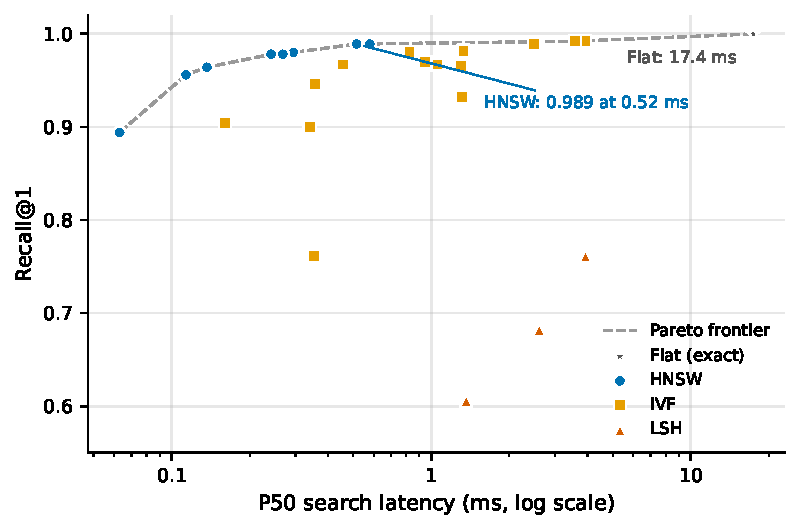
\includegraphics[width=\columnwidth]{hnsw_pareto_tradeoff}
  \caption{Recall@1 vs.\ P50 search latency (log scale) for all
  index configurations on 499K vectors, uniform workload. HNSW
  traces the Pareto frontier up to Recall@1 $=$ 0.989 at 0.52 ms;
  exact Flat search pays 17.4 ms for perfect recall.}
  \label{fig:hnsw}
\end{figure}

\subsection{Adaptive Routing}
The adaptive router identifies a practical operating region around $\theta \in [0.76, 0.79]$. In five-seed evaluation under random cache fill, the mean selected threshold is $\theta = 0.772 \pm 0.015$, yielding a 60.43\% hit rate, average cosine quality of 0.806, and 60.33\% latency savings. The full sweep (Fig.~\ref{fig:router}) shows why the router settles in this region: hit rate and latency savings rise together as the threshold loosens, while the mean cosine similarity of accepted hits falls. Beyond $\theta = 0.90$, additional hits come almost entirely from low-quality accepts; the mean accepted-hit cosine drops from 0.76 at $\theta = 0.9$ to 0.69 at $\theta = 1.5$, where every query is accepted.

\begin{figure}[t]
  \centering
  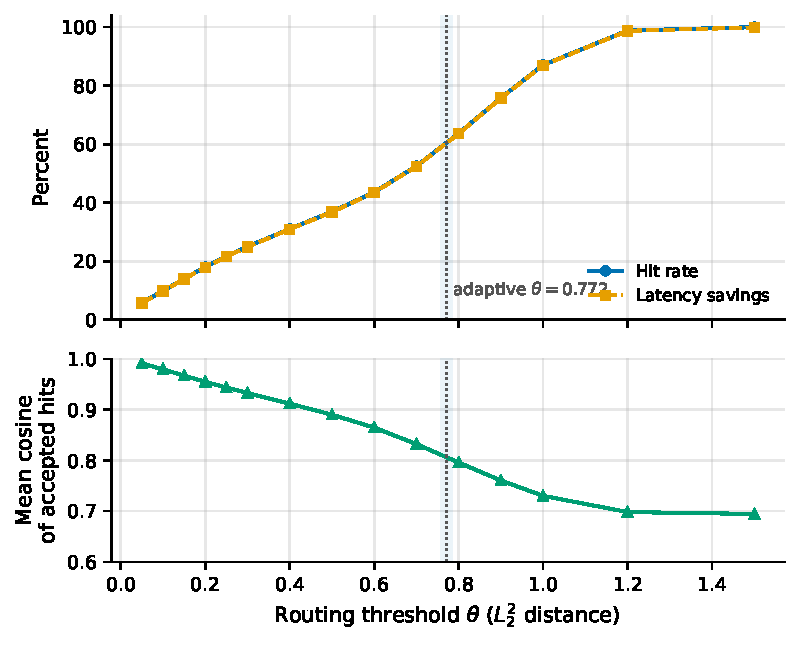
\includegraphics[width=\columnwidth]{router_threshold_sweep}
  \caption{Five-seed mean threshold sweep under random cache
  fill. Hit rate and latency savings rise as the threshold
  loosens while accepted-hit quality falls; the adaptive router
  settles at $\theta = 0.772 \pm 0.015$ (shaded band).}
  \label{fig:router}
\end{figure}

\subsection{Cache Eviction Performance}
The semantic eviction policy provides no hit-rate benefit on the LMSYS workload (Fig.~\ref{fig:eviction}). Table~\ref{tab:hit-rate} reports hit rates for LRU, LFU, and the semantic policy on the full 579,753-query stream. At 10\% capacity, LFU leads the semantic policy by 0.27\,pp and LRU by 0.33\,pp; at 20\% and 30\% capacity, all three policies agree to four decimal places. Seed variance is below reporting precision, so these small differences are stable, but they carry no practical significance.

\begin{table}[t]
\caption{Cache hit rate (mean $\pm$ std) across three seeds
(42, 123, 456) at three cache capacities. Differences across
policies are statistically negligible at all cache sizes.}
\label{tab:hit-rate}
\resizebox{\columnwidth}{!}{%
\begin{tabular}{lccc}
\toprule
Cache Size & LRU & LFU & Semantic \\
\midrule
10\% & $0.7802 \pm 0.0001$ & $\mathbf{0.7835 \pm 0.0000}$
     & $0.7808 \pm 0.0000$ \\
20\% & $0.8453 \pm 0.0000$ & $0.8453 \pm 0.0000$ & $0.8453 \pm 0.0000$ \\
30\% & $0.8756 \pm 0.0000$ & $0.8756 \pm 0.0000$
     & $0.8756 \pm 0.0000$ \\
\bottomrule
\end{tabular}%
}
{\footnotesize $\dagger$ All stds $<$ 0.00005 except LRU at
10\% (std\,$=$\,0.00005); all round to $\pm$0.0000 or
$\pm$0.0001 as shown. Variance is non-zero but below
reporting precision.}
\end{table}

\paragraph{Runtime overhead.}
Table~\ref{tab:latency} reports mean per-query processing time for the same runs.

\begin{table}[t]
\caption{Mean per-query processing time across three seeds.
Semantic/LRU reports multiplicative overhead relative to LRU.}
\label{tab:latency}
\small
\begin{tabular}{@{}lcccc@{}}
\toprule
Cache Size & LRU & LFU & Semantic & Sem./LRU \\
\midrule
10\% & 1.45 ms & 2.53 ms & 8.47 ms & $5.83\times$ \\
30\% & 1.90 ms & 3.67 ms & 15.70 ms & $8.24\times$ \\
\bottomrule
\end{tabular}
\end{table}

In the same runs, semantic policy statistics report mean eviction computation times of 25.75 ms (10\% cache) and 90.27 ms (30\% cache). Together with the per-query overhead above, this confirms that semantic eviction is substantially more expensive while yielding no hit-rate gain.

\begin{figure}[t]
  \centering
  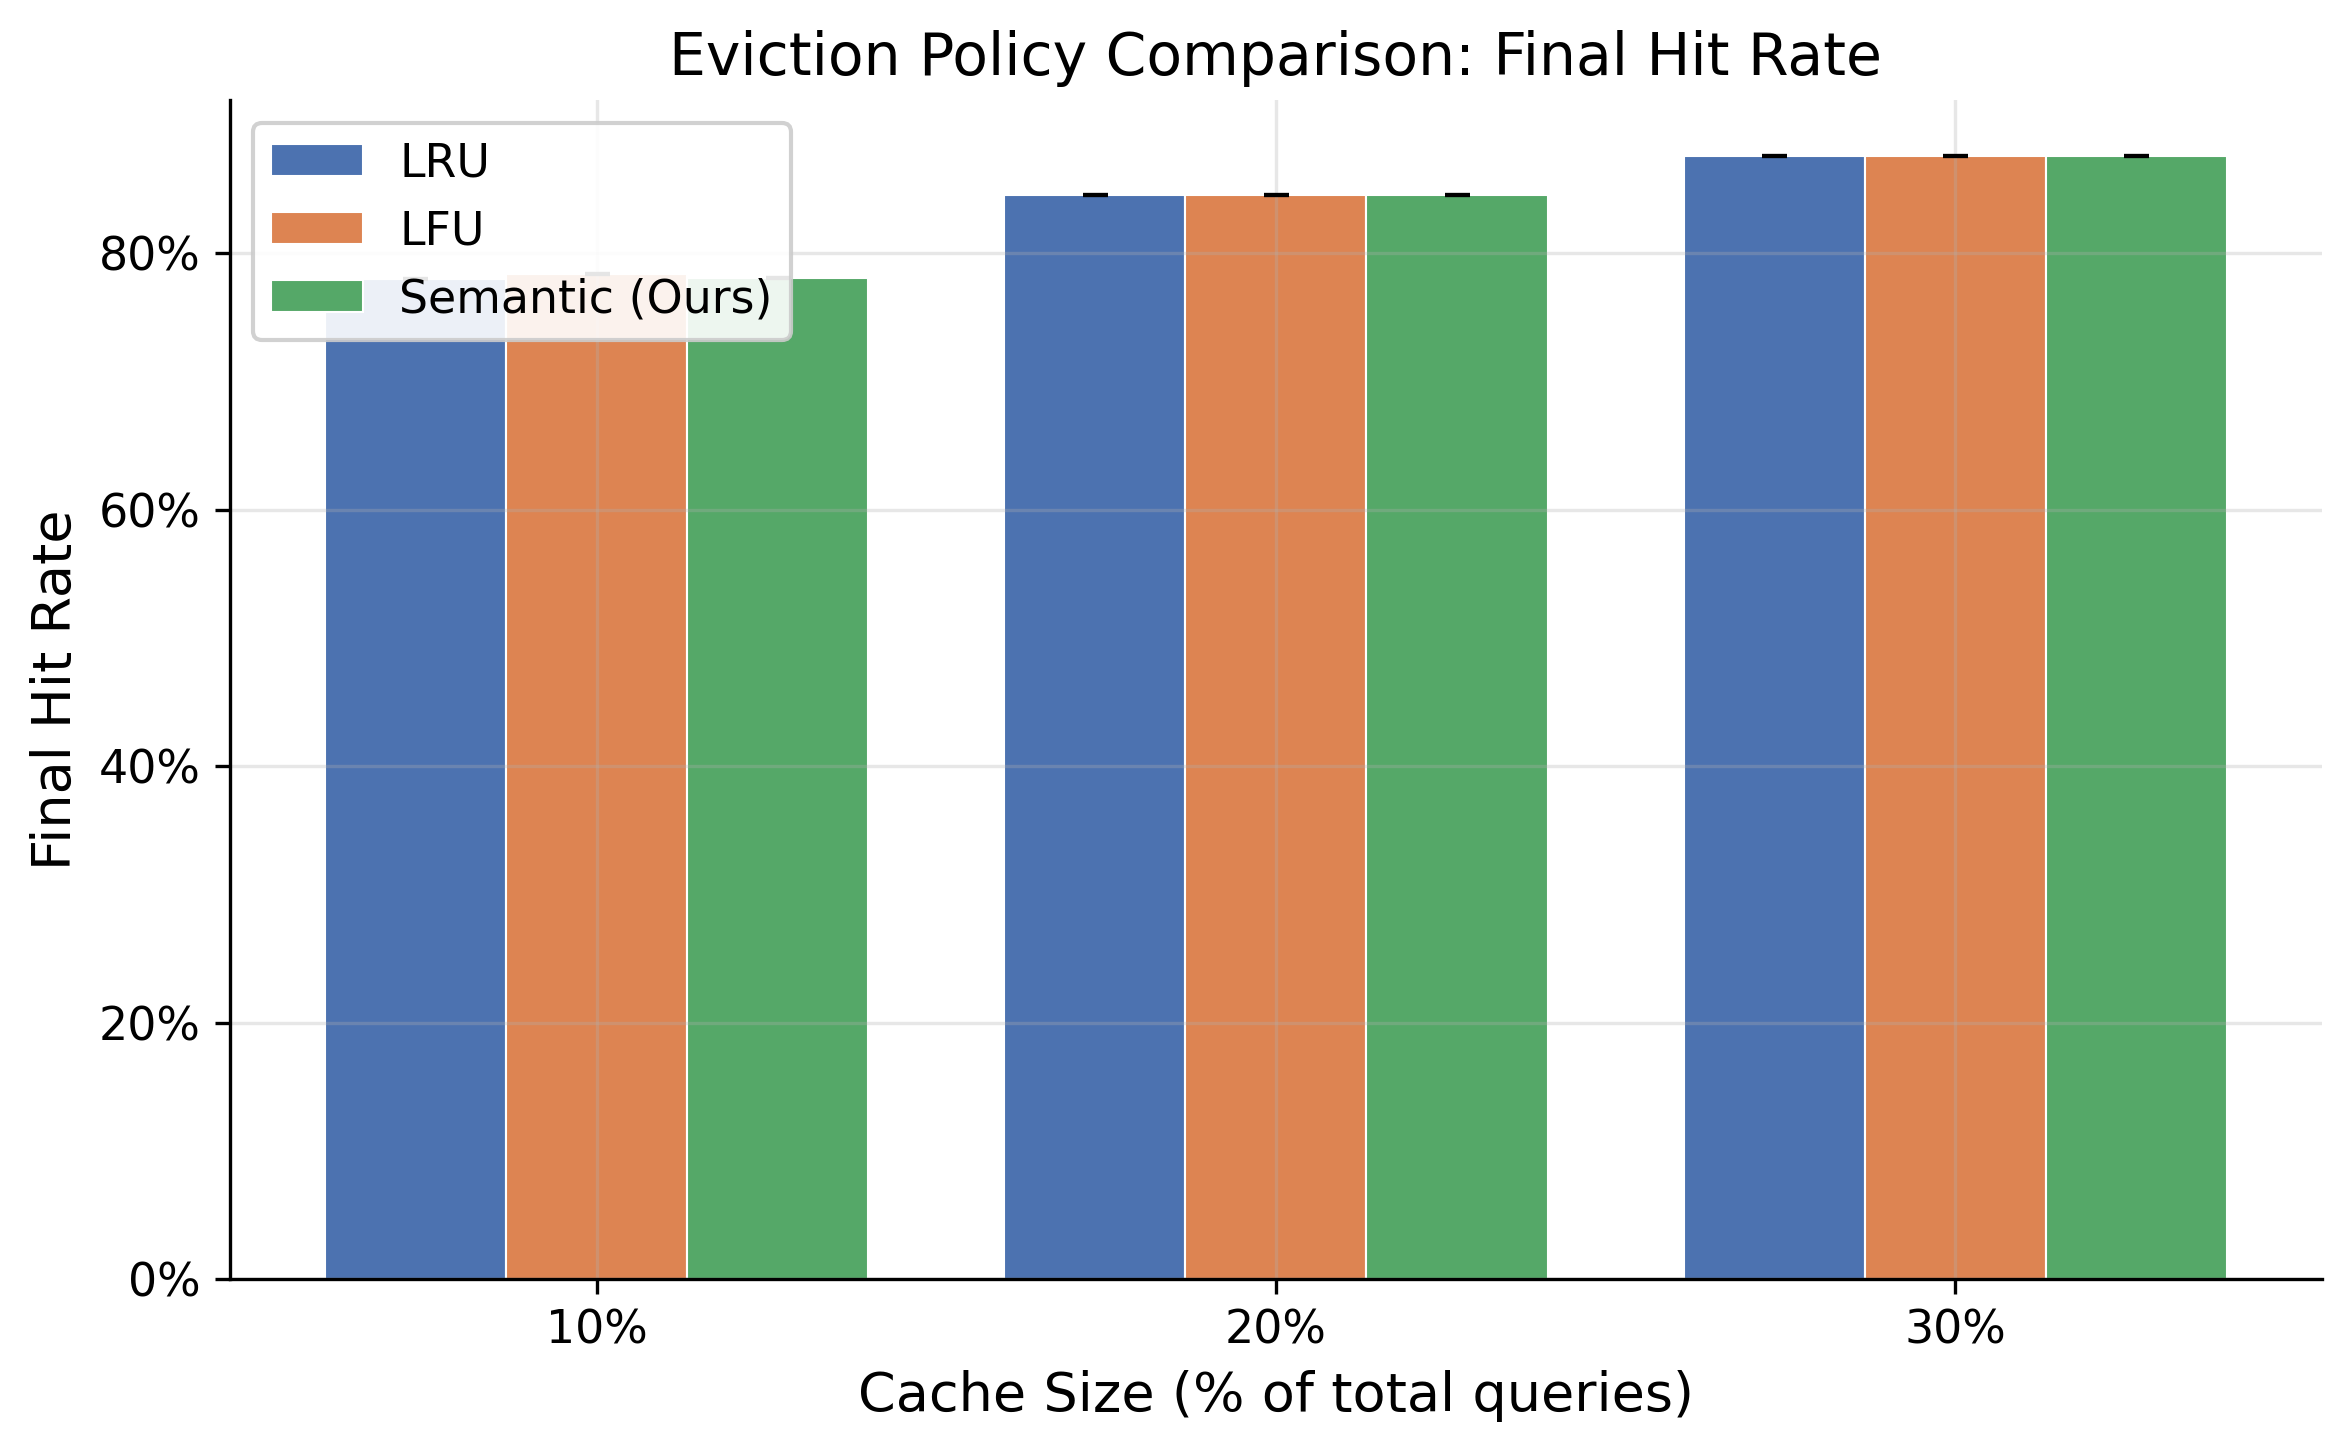
\includegraphics[width=0.88\columnwidth]{eviction_policy_comparison}
  \caption{Hit rate across eviction policies at three cache
  capacities. All three policies converge to statistically
  equivalent performance.}
  \label{fig:eviction}
\end{figure}

\subsection{Seven-Policy Comparison Across Workloads and Capacities}
\label{sec:matrix}
We extend the eviction evaluation to all seven policies on three workloads, each preprocessed into a 100{,}000-query temporal stream: LMSYS-Chat-1M, QQP \cite{iyer2017qqp} (Quora question pairs), chosen as a high-redundancy workload of near-duplicate questions, and MOSS \cite{sun2024moss}, an English synthetic-instruction corpus whose templated queries saturate any cache and serve as a control. Cache capacities are 10\%, 20\%, and 30\% of the stream, with three seeds (42, 123, 456) per cell. Figure~\ref{fig:heatmap} reports the full hit-rate matrix and Figure~\ref{fig:ablation} the capacity ablation.

No policy beats LFU by a meaningful margin. Across all eighteen dataset, capacity, and encoder cells, no policy exceeds LFU's hit rate by more than 0.05\,pp; the largest margin any policy achieves over LFU anywhere in the matrix is 0.0409\,pp (GDSF on LMSYS at 20\% capacity under MiniLM), a handful of queries out of ${\sim}70$K. On the sparse workloads at 10\% capacity, LFU reaches 57.0\% (LMSYS) and 60.0\% (QQP). ARC matches LFU to within 0.01\,pp in every cell. Its adaptation parameter only moves on semantic ghost hits, which are as rare as the redundancy signal itself, so ARC degenerates to its frequency list and inherits LFU's behavior. GDSF, as predicted by its reduction to LFU-with-aging, trails LFU by at most 0.48\,pp (QQP, 10\%) and edges it by at most 0.04\,pp elsewhere, the aging clock's only visible effect, and is otherwise indistinguishable.

At the bottom of the ranking, FIFO behaves as a weakest-baseline control should. It trails LFU by 6.33, 3.97, and 1.22\,pp on LMSYS and by 8.67, 4.64, and 0.94\,pp on QQP at 10\%, 20\%, and 30\% capacity under MiniLM, with the same pattern under gte-base. It does not beat LRU in any of the eighteen cells, and it ranks sixth or seventh of seven in seventeen of them; the single exception is a saturated MOSS cell in which all seven policies sit within 0.014\,pp of one another. Recency and frequency information therefore does carry value on these workloads, which is worth stating explicitly because it is the point on which our measurements diverge from Sun et al.\ \cite{sun2026solar}, who report FIFO outperforming LRU and LFU on semantic workloads drawn from agent memory benchmarks. The divergence is not a contradiction in measurement so much as a difference in what is being cached: their buffers hold an agent's accumulated experience, where repeated access to the same stored item is rare, whereas a serving trace repeats popular queries often enough for frequency counts to be informative at tight capacities.

SISO, the one policy in our set designed specifically for LLM caches, is the weakest performer on both sparse datasets at every capacity, trailing LFU by 6.34, 4.18, and 1.40\,pp on LMSYS and by 8.55, 4.66, and 0.96\,pp on QQP at 10\%, 20\%, and 30\% capacity. Its cluster-size signal suffers the same sparsity collapse as our semantic policy, while its maintenance rounds discard the frequency history that LFU exploits. Adding FIFO to the comparison sharpens this considerably. Across the twelve LMSYS and QQP cells, SISO and FIFO differ by 0.096\,pp on average and by at most 0.254\,pp, against a seed standard deviation of 0.006\,pp, so SISO is performing at the level of evicting in arrival order. In nine of those twelve cells, including all six LMSYS cells, SISO is measurably worse than FIFO. A policy that consults embedding geometry, maintains clusters, and costs $3.1$--$3.5\times$ LRU's per-query time thus recovers less on these workloads than a policy that ignores the embeddings entirely.

Both deficits shrink monotonically with capacity, and the same convergence applies at the top of the ranking: LFU's lead over LRU falls from 1.5\,pp (LMSYS) and 2.5\,pp (QQP) at 10\% capacity to 0.2\,pp at 20\% and to at most 0.012\,pp at 30\%. Capacity, not policy, dominates hit rate (Fig.~\ref{fig:ablation}); as the cache grows, every policy gap collapses toward zero.

MOSS behaves as intended for a control: all seven policies land between 97.6\% (10\%) and 98.7\% (30\%), within 0.02\,pp of one another at each capacity, because a saturated cache is uninformative for policy ordering. Seed variance is negligible throughout: the maximum hit-rate standard deviation across all 126 policy cells is $3.1 \times 10^{-4}$ (0.03\,pp), and $2.2 \times 10^{-4}$ within the MiniLM half, so the orderings above are essentially deterministic. SISO's hit-rate deficit is not compensated by lower cost either. At 10\% capacity, its mean stream-processing time is $3.5\times$ LRU's on LMSYS and $3.1\times$ on QQP, with our semantic policy at $4.3\times$ and $3.8\times$ respectively; only on saturated MOSS, where evictions are rare, does the overhead collapse (SISO $1.3\times$ LRU).

\begin{figure}[t]
  \centering
  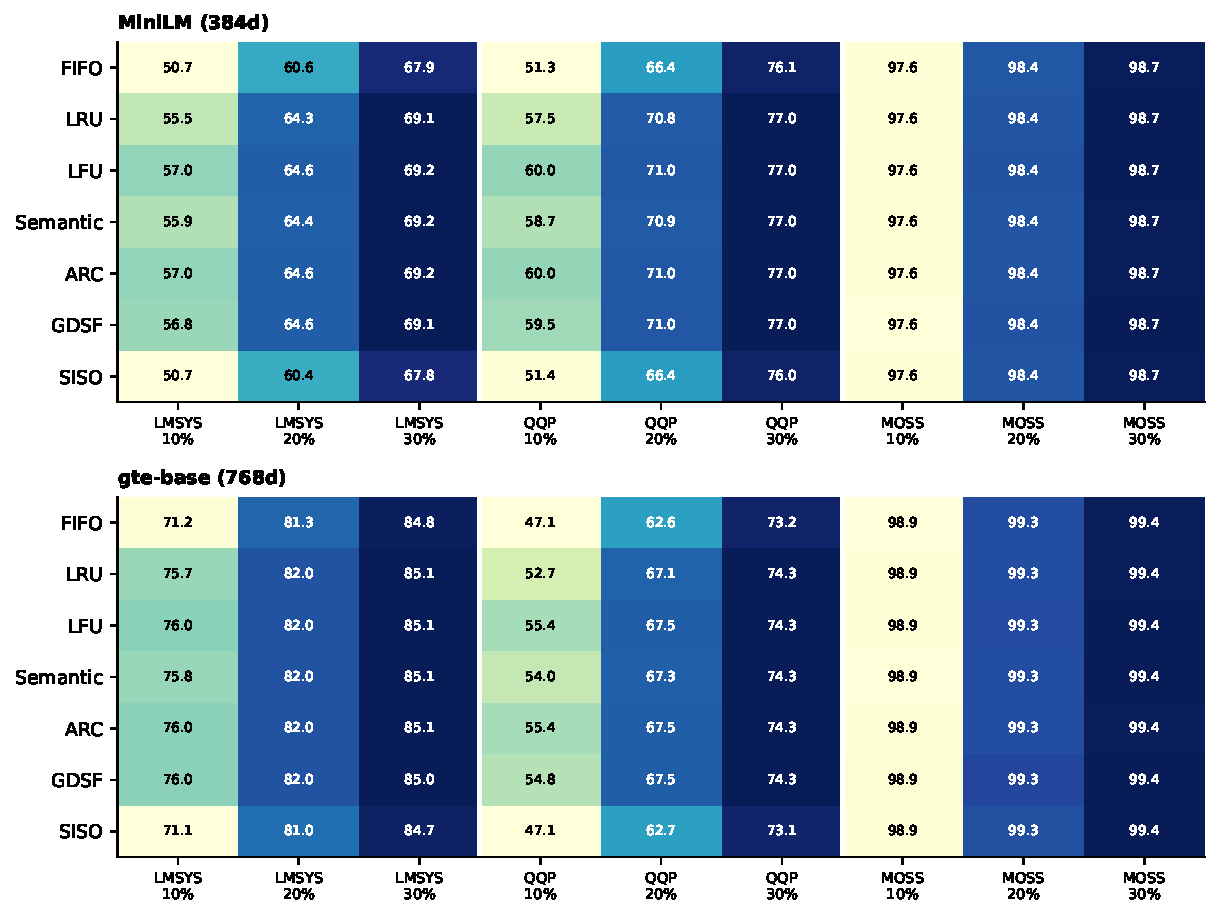
\includegraphics[width=\columnwidth]{phase6_policy_heatmap}
  \caption{Hit rate (\%) for all seven policies across three
  datasets and three cache capacities, MiniLM (top) and
  gte-base (bottom) embeddings; color is normalized within
  each dataset block. LFU is never beaten by more than
  0.05\,pp. SISO is weakest in every LMSYS and QQP cell, and
  its row is nearly indistinguishable from the FIFO control.}
  \label{fig:heatmap}
\end{figure}

\begin{figure}[t]
  \centering
  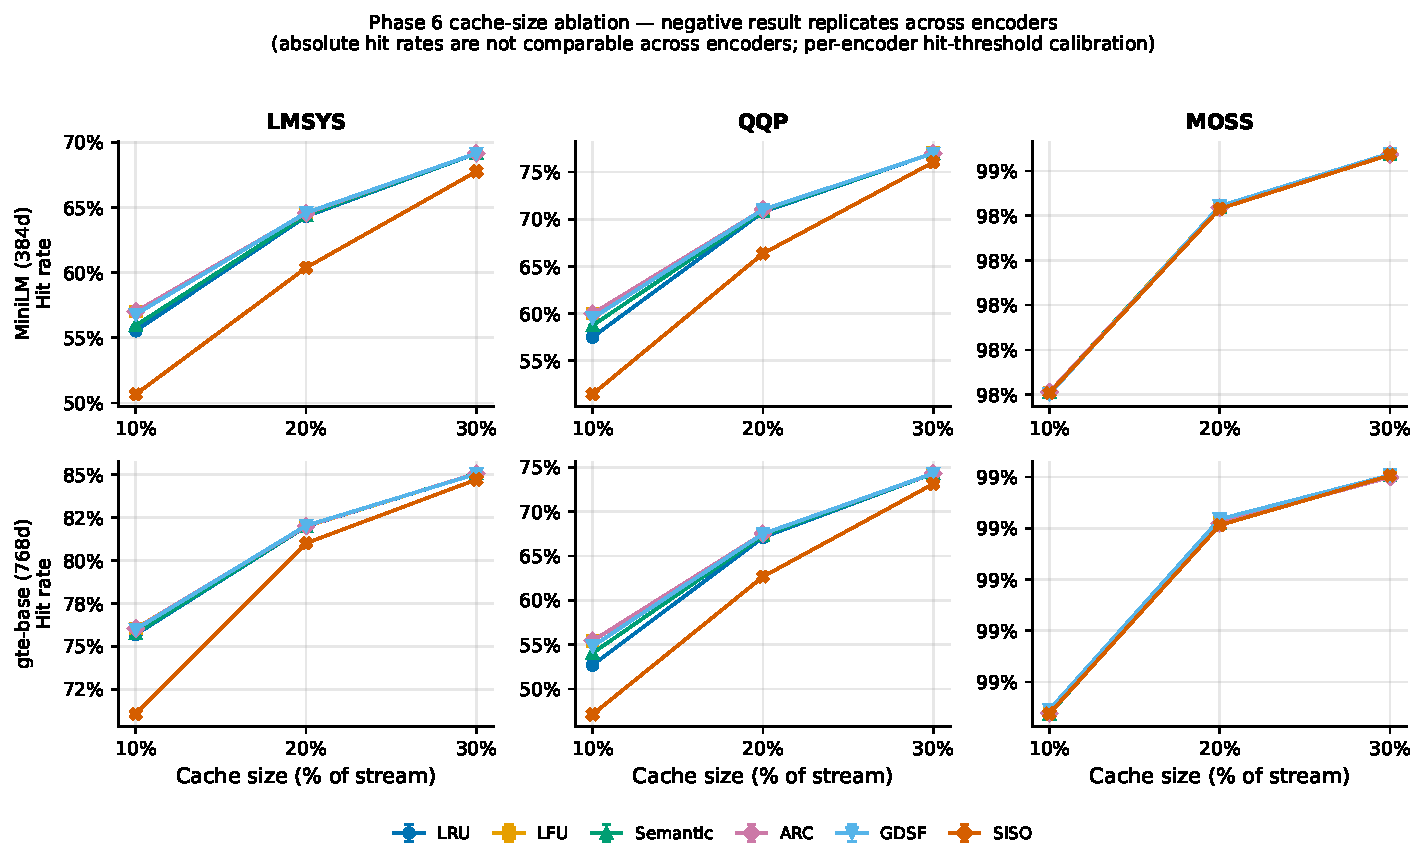
\includegraphics[width=\columnwidth]{phase6_cache_size_ablation}
  \caption{Cache-size ablation. Hit rate is governed by
  capacity, not policy: all policy gaps, including SISO's
  deficit and LFU's lead over LRU, shrink monotonically as
  the cache grows. The ordering replicates across both
  embedding encoders.}
  \label{fig:ablation}
\end{figure}

\subsection{Cross-Encoder Replication}
\paragraph{Hit thresholds do not transfer across encoders.}
Running the gte-base matrix under the MiniLM-calibrated threshold ($0.90$
$L_2^2$) is degenerate: on all three datasets, all three seeds, and all six
policies evaluated at the time (the later FIFO runs use only the
recalibrated configuration), the final hit rate is exactly $1.0$ with zero
misses and zero evictions. Because gte-base's random-pair similarity exceeds the threshold,
every query ``hits'' whatever the cache contains, eviction never fires, and
the experiment measures nothing. We report this as a methodological result:
a semantic-cache deployment that swaps encoders without recalibrating its
threshold silently degrades into serving arbitrary responses at a perfect
measured hit rate.

\paragraph{Recalibrated replication.}
After per-encoder recalibration, the policy convergence replicates exactly. At
$10\%$ capacity the policy ordering on LMSYS and QQP is identical to MiniLM's:
$\text{ARC}=\text{LFU} > \text{GDSF} > \text{Semantic} > \text{LRU}$, with
SISO and FIFO at the bottom. ARC and LFU are indistinguishable, matching within $0.01$pp in
all nine dataset--capacity cells. The semantic policy again never beats LFU by more than $0.01$pp.
SISO and the FIFO control are again the only policies that separate, and
again in the wrong direction: SISO trails the best policy by
$5.0$/$1.0$/$0.3$pp on LMSYS and $8.3$/$4.8$/$1.2$pp on QQP at $10/20/30\%$
capacity, with FIFO tracking SISO to within $0.3$\,pp throughout; both
deficits narrow as capacity grows. The LFU--LRU frequency advantage likewise shrinks with
capacity ($+2.7$/$+0.4$/$+0.0$pp on QQP; $+0.4$/$+0.0$/$+0.0$pp on LMSYS),
and MOSS remains saturated for every policy ($0.989$--$0.994$ hit rate, fewer
than $750$ mean evictions). Figure~\ref{fig:ablation} shows both encoder rows.

\paragraph{Orderings transfer; absolute rates do not.}
While the ranking of policies is encoder-robust, absolute hit rates are not:
at $10\%$ capacity, LFU achieves $0.760$ on LMSYS under gte-base versus
$0.570$ under MiniLM ($+19.0$pp), yet $0.554$ versus $0.600$ on QQP
($-4.6$pp). The differences are large and not even direction-consistent,
so hit rates measured under one encoder cannot be used to provision a cache
served by another. What does transfer is the relative conclusion:
frequency-based eviction dominates, and semantic and workload-aware
alternatives add cost without benefit.

\subsection{Quality-Adjusted Hit Rate}
\begin{table*}[t]
\caption{Judged hit quality at 10\% cache (MiniLM, seed 42): raw hit
rate (\%), judged-equivalent (YES) fraction with Wilson 95\% CI
($n{=}1000$ per cell), and quality-adjusted hit rate
QA $=$ Raw $\times$ YES (\%). Within every dataset the YES intervals
of all six policies overlap.}
\label{tab:judge}
\centering
\small
\begin{tabular}{l rrr rrr rrr}
\toprule
 & \multicolumn{3}{c}{LMSYS} & \multicolumn{3}{c}{QQP} & \multicolumn{3}{c}{MOSS} \\
Policy & Raw & YES [95\% CI] & QA & Raw & YES [95\% CI] & QA & Raw & YES [95\% CI] & QA \\
\midrule
LRU & 55.5 & 3.6 [2.6, 4.9] & 2.0 & 57.5 & 2.5 [1.7, 3.7] & 1.4 & 97.6 & 25.1 [22.5, 27.9] & 24.5 \\
LFU & 57.0 & 3.9 [2.9, 5.3] & 2.2 & 60.0 & 2.6 [1.8, 3.8] & 1.6 & 97.6 & 26.1 [23.5, 28.9] & 25.5 \\
Semantic & 55.9 & 3.1 [2.2, 4.4] & 1.7 & 58.7 & 3.1 [2.2, 4.4] & 1.8 & 97.6 & 26.1 [23.5, 28.9] & 25.5 \\
ARC & 57.0 & 3.3 [2.4, 4.6] & 1.9 & 60.0 & 2.6 [1.8, 3.8] & 1.6 & 97.6 & 26.1 [23.5, 28.9] & 25.5 \\
GDSF & 56.8 & 3.9 [2.9, 5.3] & 2.2 & 59.5 & 2.3 [1.5, 3.4] & 1.4 & 97.6 & 24.7 [22.1, 27.5] & 24.1 \\
SISO & 50.7 & 3.1 [2.2, 4.4] & 1.6 & 51.4 & 2.1 [1.4, 3.2] & 1.1 & 97.6 & 27.0 [24.3, 29.8] & 26.4 \\
\bottomrule
\end{tabular}

\end{table*}

\begin{figure}[t]
  \centering
  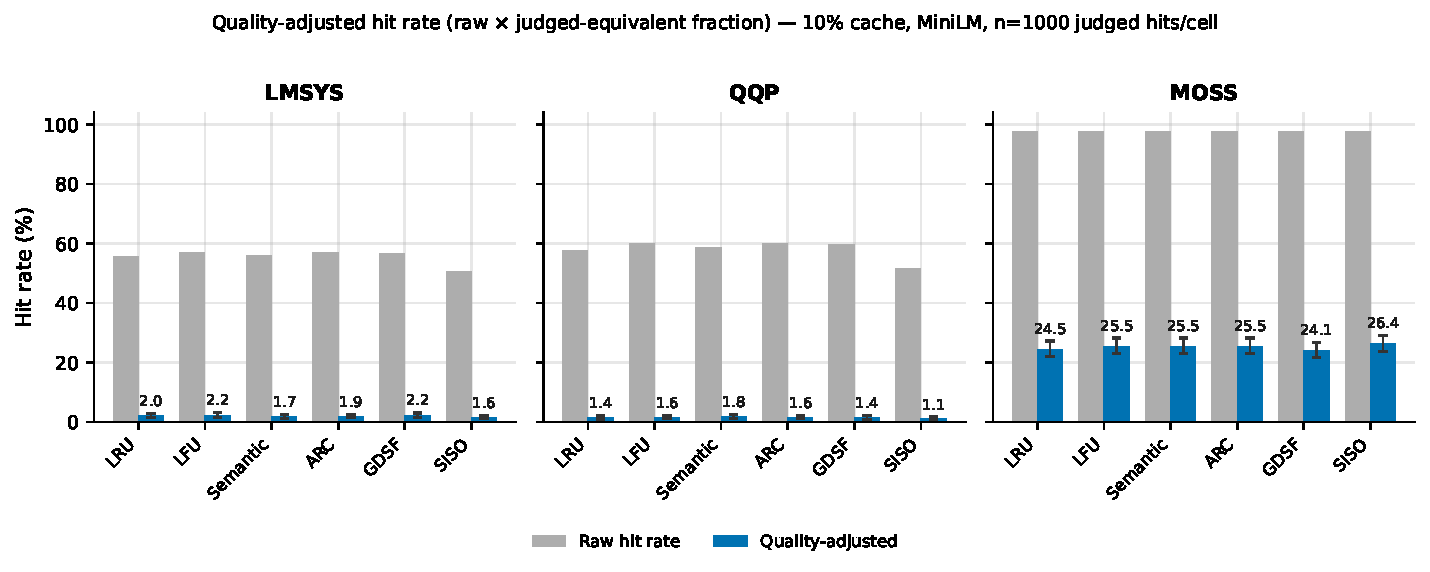
\includegraphics[width=\columnwidth]{judge_quality_adjusted}
  \caption{Raw vs.\ quality-adjusted hit rate per dataset and policy.
  Quality adjustment collapses LMSYS and QQP hit rates by more than an
  order of magnitude and erases the ordering among policies.}
  \label{fig:qadj}
\end{figure}

\begin{figure}[t]
  \centering
  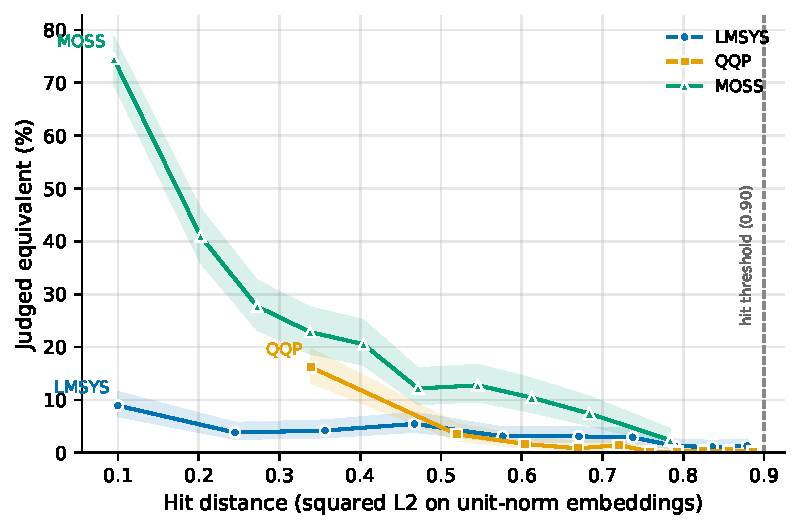
\includegraphics[width=\columnwidth]{judge_yes_vs_distance}
  \caption{Judged equivalence rate vs.\ $L_2^2$ hit distance (decile
  bins of unique pairs, Wilson 95\% CIs). MOSS decays steeply; QQP has
  no near-duplicate regime; LMSYS stays low even at near-zero
  distance due to templated prompts.}
  \label{fig:yesdist}
\end{figure}

Table~\ref{tab:judge} and Figure~\ref{fig:qadj} show the central
result: at the 0.90 hit threshold, most of the matches counted by the
raw hit rate do not answer the incoming query.
On LMSYS, raw hit rates of 50.7--57.0\% shrink to quality-adjusted
rates of 1.6--2.2\% (judged-YES fractions of 3.1--3.9\%); on QQP,
51.4--60.0\% shrinks to 1.1--1.8\% (YES 2.1--3.1\%). Even on MOSS, the
clustered workload where every policy hits 97.6\%, only 24.7--27.0\%
of sampled hits are judged equivalent, for quality-adjusted rates of
24.1--26.4\%.

Quality adjustment also flattens the policy ordering. Within each
dataset, the Wilson 95\% intervals on the YES fractions of all six
policies overlap (Table~\ref{tab:judge}), so at $n{=}1000$ per cell
the observed spreads are indistinguishable from binomial noise. The
inversion on MOSS is illustrative: SISO, the worst policy by raw hit
rate on the other datasets, attains the numerically highest YES rate
(27.0\%). Rapid turnover costs nothing when the entries a careful
policy would have retained produce mostly non-equivalent hits anyway.

Figure~\ref{fig:yesdist} shows the mechanism behind these numbers:
judged equivalence decays with embedding distance, and the shape of
the decay differs across datasets. MOSS falls from
74.5\% YES in its nearest distance decile to 2.4\% in its farthest.
QQP has no near-duplicate regime at all: its nearest decile already
sits at median $L_2^2 = 0.34$ with only 16.2\% YES. LMSYS is the
starkest case. Even its nearest decile (median $L_2^2 = 0.10$) yields
only 8.9\% YES, with mid-range deciles at 3--5\%. Manual inspection
attributes this to MiniLM saturating on long templated prompts:
pairs at near-zero distance share an instruction template
(e.g., ``You are the text completion model\ldots'') but differ in the
payload the template wraps, and the judge correctly rejects them.
Near-zero embedding distance therefore does not guarantee equivalence.

The verdicts are stable across judge runtimes. On the 1{,}931-pair
overlap between the local Ollama judge and Groq's hosted
\texttt{llama-3.1-8b-instant}, raw agreement is 98.55\% with Cohen's
$\kappa = 0.826$; the 28 disagreements concentrate at close distances
(median $L_2^2$ 0.236 vs.\ 0.606 for agreements), i.e., genuinely
borderline pairs. Because 1{,}923 of the overlap pairs are from
LMSYS, this validation speaks primarily to the LMSYS verdicts.

\section{Discussion: Why the Policies Converge}
The convergence reported above is consistent enough across workloads, capacities, and encoders that it demands a mechanism rather than a case-by-case explanation, and this section supplies one. We show that the redundancy signal a semantic policy needs is suppressed by the cache's own admission rule, trace the consequences through the scoring function, and then translate the measurements into deployment guidance.

\subsection{The Sparsity of the Redundancy Graph}
The LMSYS dataset is characterized by high entropy. Distance-distribution analysis (Fig.~\ref{fig:distance}) shows weak local clustering under the routing and eviction thresholds used in our experiments.

Across all semantic runs (3 seeds $\times$ cache sizes 10\%, 20\%, 30\%), the mean redundancy per run ranges from $2.2\text{--}2.9 \times 10^{-5}$, with maximum observed redundancy 0.035. This is still substantially below the smoothing constant $\mu = 0.1$, so the $\mu$ term dominates the numerator and the scoring function reduces to inverse-utility ordering for most entries.

\begin{figure}[t]
  \centering
  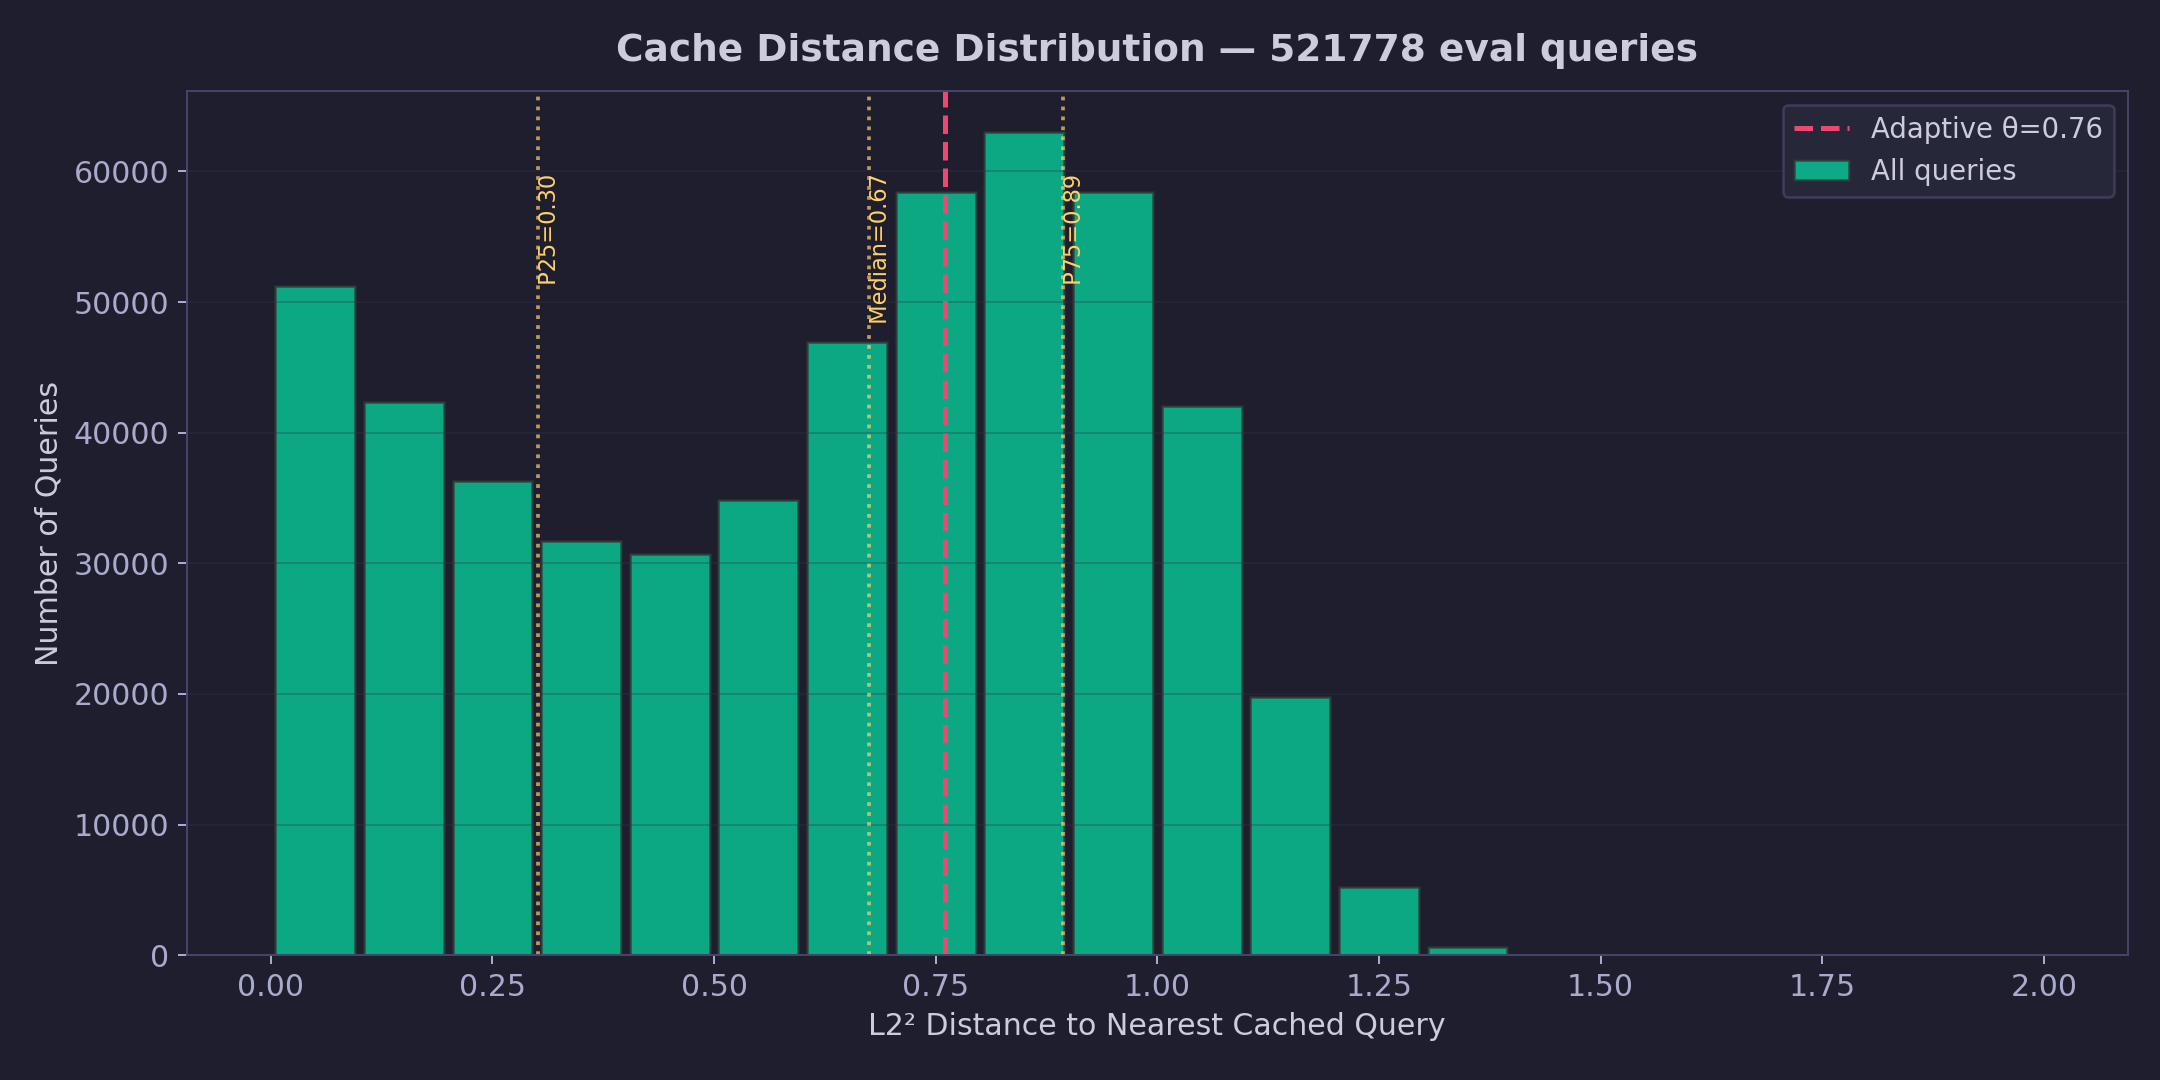
\includegraphics[width=0.88\columnwidth]{lmsys_distance_distribution}
  \caption{Pairwise $L_2^2$ distance distribution for LMSYS
  query embeddings. Most pairs exceed the routing threshold,
  explaining redundancy graph sparsity.}
  \label{fig:distance}
\end{figure}

\subsection{Cache-Content Density Characterization}
To locate where the redundancy signal vanishes, we profile density over the
cache contents rather than the workload: at periodic snapshots of the
reference LRU cache during the stream ($10\%$ capacity, MiniLM), we measure
the mean fraction of cached entries within $L_2^2$ distance $\theta$ of each
cached entry.

Figure~\ref{fig:density} shows the result. At the eviction threshold
$\theta = 0.90$, cache-content density orders QQP $<$ LMSYS $<$ MOSS
($2.1\times10^{-5}$, $4.1\times10^{-4}$, $2.5\times10^{-3}$ at the final
checkpoint); at $\theta = 0.30$, QQP's cache density falls to zero. This
inverts the workload-level expectation. QQP, built from duplicate-question
pairs, is the most redundant workload, and it shows the largest
LFU--LRU frequency payoff ($+2.49$pp, versus $+1.47$pp for LMSYS and
$+0.00$pp for saturated MOSS). Yet its cache contents are the
sparsest, $20\times$ below LMSYS and two orders of magnitude below MOSS.

The mechanism is self-deduplication. A query within $\theta$ of a cached
entry is a hit and is never inserted, so the cache accumulates precisely the
residue of mutually distant queries; the denser the workload, the more
aggressively the admission rule filters its redundancy out. Because the
semantic policy's neighbor threshold equals the hit threshold, the very
signal it evicts by is structurally suppressed by the cache it manages.
Even MOSS's peak density ($2.5\times10^{-3}$) sits $40\times$ below the
smoothing constant $\mu = 0.1$, so the scoring function collapses to
inverse-utility ordering on every dataset. The convergence is
therefore not an artifact of LMSYS's diversity; a semantic cache starves its
own eviction policy of the redundancy signal on any workload.
\begin{figure}[t]
  \centering
  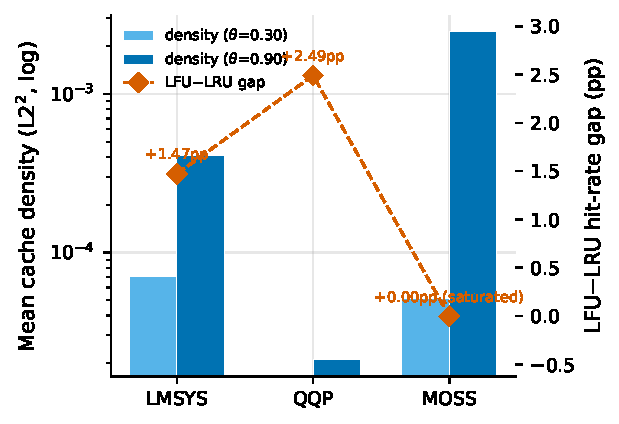
\includegraphics[width=\columnwidth]{density_characterization}
  \caption{Mean cache-content density (log scale) at $L_2^2$
  $\theta = 0.30$ and $0.90$, with the LFU$-$LRU hit-rate gap
  (right axis) at $10\%$ capacity. QQP, the most redundant
  workload, yields the sparsest cache: hits are never inserted,
  so the cache self-deduplicates.}
  \label{fig:density}
\end{figure}

\subsection{Mathematical Degradation to LFU}
When $r(e) = 0$, the numerator of our scoring function collapses to the smoothing constant $\mu$. The equation simplifies to:
\begin{equation}
\mathit{score}(e) = \frac{\mu}{\mathit{utility}(e)}
\end{equation}
Because $\mu$ is a constant, the cache entries are ranked entirely by inverse-utility. The semantic policy then behaves exactly like a slightly heavier LFU/LRU hybrid.

\subsection{The Necessity of $\mu$-Smoothing}
\label{sec:mu}
While $\mu$-smoothing caused the policy to degrade to LFU, this degradation is a necessary safeguard. Without $\mu$ (i.e., $\mu=0$), any entry with no neighbors ($r(e)=0$) would receive a score of exactly 0. This entry would become ``immortal,'' permanently occupying a cache slot regardless of how rarely it is accessed. $\mu$ ensures the cache remains functional and degrades gracefully to a proven baseline when the semantic signal fails.

\subsection{Which Policy Should a Deployment Use?}
\label{sec:guidance}

The measurements support a short decision procedure.

\paragraph{Default to LFU.} On every workload, capacity, and encoder we tested, LFU is either the best policy or within 0.05\,pp of it, and it is among the cheapest to run. Nothing in our results justifies deploying a more complex policy by default. ARC is a defensible alternative on the same evidence, since it matches LFU to within 0.01\,pp everywhere, but it converges to LFU's decisions rather than improving on them, so the added implementation cost buys nothing here.

\paragraph{Capacity matters more than policy.} If the cache can be enlarged, that is the intervention with real returns. The LFU--LRU gap falls from 2.5\,pp at 10\% capacity to below 0.01\,pp at 30\% on QQP, and every other policy gap collapses on the same schedule. For a team weighing eviction tuning against provisioning a larger cache, the larger cache returns more. Policy choice matters only in the capacity-constrained regime, and even there the margins are small.

\paragraph{Measure cache-content density before adopting a semantic policy.} Semantic eviction is not universally ineffective, but its applicability condition is specific and testable: the redundancy of the cache contents under the intended threshold, not the redundancy of the workload, must be substantial relative to the smoothing constant $\mu$. Our density profiles put every workload we tested at least $40\times$ below $\mu = 0.1$, including MOSS at its densest. The check is cheap, requires no LLM calls, and should precede any adoption decision. Workloads plausibly dense enough to pass it include repetitive corporate FAQ systems, automated homework or coding assessment platforms, and domain-specific RAG pipelines with constrained query vocabularies. General-purpose conversational deployments will not pass it.

\paragraph{Budget for the overhead if adopting one anyway.} The semantic policy costs $5.83$--$8.24\times$ LRU's per-query time and SISO costs $3.1$--$3.5\times$, against hit-rate differences at or below 0.05\,pp in the favorable direction and up to $8.5$\,pp in the unfavorable one. A policy that reasons about embedding geometry must recompute neighbor relations as the cache mutates, and that cost is incurred on every eviction regardless of whether the signal is present.

\paragraph{Spend the effort on thresholds and audits instead.} The two decisions that changed outcomes by orders of magnitude in this study were the similarity threshold and what counts as a valid hit. Recalibrating a threshold per encoder is a one-time offline procedure, and judged spot-checks of sampled hits are inexpensive relative to the serving costs they protect. Both dominate any eviction-policy decision available to a practitioner today.

\subsection{What Quality Adjustment Means for the Policy Comparison}
\label{sec:qadj-meaning}
The judge results strengthen the convergence finding in two ways.
First, the eviction policies are tied not only on raw hit rate but
also on judged equivalence, since no policy's judged-equivalence
fraction separates from the others beyond binomial noise. Second, the
raw hit rates the policies were competing over are largely illusory:
at the 0.90 threshold, roughly 96--97\% of LMSYS and QQP hits would
return an answer to a different question. The decisive design choice
in a semantic cache is therefore admission rather than eviction. The
hit threshold and the quality of the match signal determine how much
value the cache can deliver before any eviction decision is made.
Verified caching reaches the same conclusion from the design side,
replacing the single global threshold with per-entry thresholds under an
explicit error budget \cite{schroeder2025vcache}.
This finding also bears on the router's quality proxy. The
router scores hits by cosine similarity ($1 - d^2/2$), yet the
templated-prompt failure shows that cosine similarity can approach 1.0
on pairs a judge deems non-equivalent, so similarity is an unreliable
stand-in for answer quality on boilerplate-heavy text. Consequently, the
60.33\% latency savings (Fig.~\ref{fig:router}) are reported at a cosine
operating point that our judge audit does not directly cover, since the audit
fixes the eviction hit threshold ($0.90$ $L_2^2$) rather than the tighter
router-selected $\theta = 0.772$. Because the router threshold is stricter,
however, every hit the router would accept already lies inside the judged
sample, and a distance-conditioned reanalysis bounds what a dedicated audit
would find. Restricting the deduplicated judged LMSYS pairs to distances at
or below the router threshold yields a judged-equivalence rate of 4.5\%
($n = 3{,}912$; Wilson 95\% CI 3.9--5.1\%), against 3.5\% for the full
0.90-threshold sample
(\texttt{scripts/21\_judge\_router\_threshold.py --reanalyze-existing}).
The tighter operating point therefore does not restore hit quality on its
own, and most of the routed latency savings are realized on hits a judge
deems non-equivalent. This reanalysis conditions on the hit distribution of
the 0.90-threshold runs rather than re-simulating cache dynamics at
$\theta = 0.772$; the full judged, response-grounded audit at the router's
operating point, scaffolded in the same script, remains future work.

\section{Limitations}

This study has several limitations. First, both embedding models are compact sentence encoders (\texttt{all-MiniLM-L6-v2}, 384 dimensions; \texttt{gte-base}, 768 dimensions). The cross-encoder replication shows the policy ordering is robust, but larger embedding models may produce different distance geometry, and our own results show that absolute hit rates do not transfer across encoders. Second, the three datasets, while spanning diverse and redundant workloads, are all English-language chatbot or question corpora; results may not generalize to specialized workloads such as code or domain-specific RAG. Third, latency benchmarks were conducted on CPU-only hardware; GPU-accelerated serving infrastructure may shift the relative overhead of semantic eviction. Fourth, multi-turn conversation context was excluded from the cache key, treating each turn as independent; context-aware caching \cite{yan2025contextcache} may yield different hit-rate characteristics. Fifth, the judge itself is an 8B-parameter model and may misjudge subtle equivalences, although the near-identical verdicts from an independent hosted runtime ($\kappa = 0.826$) indicate the findings are not an artifact of one deployment. Sixth, query equivalence is a proxy for the quantity we ultimately care about, response reusability: a non-equivalent query pair can occasionally share a serviceable answer. Finally, the judged sample covers the seed-42 MiniLM runs at 10\% cache capacity only, and predates the FIFO runs, so the quality-adjusted rates are point estimates for one operating configuration across six of the seven policies rather than seed-averaged quantities over the full matrix.

\section{Conclusion}
We set out to determine which cache eviction policy an LLM serving deployment should use, and we answered it by running the candidates against each other on a common harness rather than comparing published numbers from incomparable settings. The answer is LFU, and the more useful finding is how little that choice matters. Across three workloads, three capacities, two encoders, and three seeds, no policy beats LFU by more than 0.05\,pp, ARC converges to LFU's decisions rather than improving on them, GDSF reduces to LFU-with-aging, and SISO, the one policy in our set designed specifically for LLM serving, is the weakest performer on both sparse workloads, matching a FIFO control to within 0.1\,pp on average while costing several times more per query. Every gap shrinks monotonically as capacity grows and has effectively vanished by a 30\% cache.

The mechanism behind this convergence is what makes it generalize. Because a query that hits is served without re-insertion, the cache deduplicates itself and accumulates the residue of mutually distant entries, so the redundancy signal a semantic policy depends on is suppressed by the very admission rule that defines the cache. The most redundant workload we tested yields the sparsest cache contents. This is a property of how semantic caches work rather than of any particular corpus, which is why we expect the result to hold beyond the three workloads studied here.

Two decisions that receive far less attention than eviction dominate it. Similarity thresholds do not transfer across embedding encoders, and an uncalibrated threshold silently degrades a cache into serving arbitrary responses at a perfect measured hit rate. Admission quality dominates in turn: an LLM judge finds that most hits at the standard threshold are not semantically equivalent queries, collapsing quality-adjusted hit rates by more than an order of magnitude and erasing the differences the policies were competing over. A practitioner following our results should deploy LFU, provision capacity rather than tune replacement, recalibrate thresholds whenever the encoder changes, and audit sampled hits for validity.

Our results also disagree with a contemporaneous study that finds FIFO superior to LRU and LFU on semantic workloads \cite{sun2026solar}, which we attribute to a difference in what is cached and in the locality structure of the request stream rather than to a discrepancy in either measurement. Characterizing exactly which stream properties flip that ordering is the clearest next step. Three further questions remain open: whether combinatorial or bandit-based eviction \cite{liu2026semantic} can overcome the sparsity limit through online adaptation; whether response-grounded judging on workloads with stored responses corroborates the query-equivalence audit; and whether the quality-adjusted picture holds when the judged audit extends beyond seed 42, MiniLM, and the 10\% cache to additional seeds, capacities, the second encoder, and a stronger independent judge.
\section{Reproducibility and Artifact Availability}
All code, configuration files, and raw result artifacts are included in the accompanying repository. Each experiment is produced by a numbered driver script under \texttt{scripts/} paired with a YAML config under \texttt{configs/}, and every run writes a JSON manifest recording its exact command line, the config file and a content hash of its resolved parameters, the Python version (3.11.13) and pinned package versions (\texttt{numpy}~2.4.2, \texttt{torch}~2.10.0, \texttt{faiss}~1.14.1, \texttt{transformers}~5.1.0, \texttt{sentence-transformers}~5.2.2), the Git commit, branch, and working-tree state, the node hardware (logical/physical cores, RAM, kernel), and a UTC timestamp.

\textbf{Pipeline.} The core results are regenerated by \path{03_run_index_benchmark.py} (\path{configs/index_benchmark.yaml}); \path{06_run_routing_eval.py} \texttt{--config} \path{configs/routing.yaml} \texttt{--multi-seed} (five-seed adaptive router); \path{08_run_eviction.py} \texttt{--config} \path{configs/eviction.yaml} \texttt{--multi-seed} (three-policy full-LMSYS eviction); the seven-policy matrix via \path{08_run_eviction.py} \texttt{--size 100k} \texttt{--multi-seed}, with \texttt{--dataset} set to each of \texttt{lmsys}, \texttt{qqp}, and \texttt{moss} and \texttt{--embedding-model} to each encoder, against \path{configs/eviction.yaml} (MiniLM) and \path{configs/eviction_gte.yaml} (recalibrated gte-base), the FIFO cells produced by the same driver invoked with \texttt{--policies fifo}; and the judged-quality audit via \path{16_sample_hits_for_judge.py} $\rightarrow$ \path{17_run_llm_judge.py} $\rightarrow$ \path{18_visualize_judge.py}.

\textbf{Claim-to-artifact map.} Table~\ref{tab:artifacts} maps each headline claim to the artifact that produces it.

\begin{table}[h]
  \caption{Claim-to-artifact map. Paths are relative to the repository root.}
  \label{tab:artifacts}
  \footnotesize
  \begin{tabular}{@{}>{\raggedright\arraybackslash}p{0.42\columnwidth}>{\raggedright\arraybackslash}p{0.50\columnwidth}@{}}
    \toprule
    Claim & Artifact \\
    \midrule
    Index Pareto frontier (Fig.~\ref{fig:hnsw}) & \path{results/benchmarks/index_benchmark_*.json} \\
    Adaptive routing, 60.33\% savings at $\theta{=}0.772$ (Fig.~\ref{fig:router}) & \path{results/routing/routing_eval_multi_seed.json} \\
    Three-policy full-LMSYS eviction (Fig.~\ref{fig:eviction}, Table~\ref{tab:hit-rate}) & \path{results/eviction/eviction_results_multi_seed.json} \\
    Seven-policy matrix (Figs.~\ref{fig:heatmap},~\ref{fig:ablation}) & \path{results/eviction/phase6_matrix_*}, \path{results/eviction/phase10_fifo_*} \\
    Recalibrated gte-base replication (\S\ref{sec:calibration}) & \path{results/eviction/phase6_recal_*} \\
    Judged hit quality (Table~\ref{tab:judge}, Figs.~\ref{fig:qadj},~\ref{fig:yesdist}) & \path{results/judge/}, \path{paper/tables/phase8_judge_table.tex} \\
    Router-threshold judged quality (\S\ref{sec:qadj-meaning}) & \path{results/judge/phase7_minilm_c0p10_local/verdicts.jsonl} at $L_2^2 \le 0.772$ \\
    \bottomrule
  \end{tabular}
\end{table}

\textbf{Determinism and provenance.} Eviction cells run three seeds (42, 123, 456) and routing five (42, 123, 456, 789, 1024); the maximum hit-rate standard deviation across all policy cells is $3.1\times10^{-4}$ ($2.2\times10^{-4}$ within the MiniLM half), so orderings are effectively deterministic. The 30\% warmup prefix and per-encoder thresholds are fixed by config. Representative run commits are \texttt{39676dd} (routing), \texttt{e4f39ee} (three-policy eviction), and \texttt{d386ffa} (policy matrix; the FIFO cells record their own commits in their manifests); full per-run provenance, including working-tree state, is in each artifact's manifest. The index-benchmark artifact predates the manifest instrumentation and is regenerated deterministically from \texttt{03\_run\_index\_benchmark.py} and its config.

\section{Ethical Considerations}
This work uses the publicly released LMSYS-Chat-1M, Quora Question Pairs, and MOSS datasets and does not involve new human-subject data collection. We evaluate systems-level cache behavior rather than user-level profiling, and report aggregate metrics only. The LLM judge runs locally on open-weight models; no query content was sent to third-party services beyond a rate-limited validation subset.

\section*{Acknowledgments}
This project was conducted as part of CSE 584 (Advanced Database Systems) at the University of Michigan. We thank Professor Lin Ma for his guidance and feedback throughout the course and this project. We also thank the creators of the LMSYS-Chat-1M, Quora Question Pairs, and MOSS datasets, and acknowledge the University of Michigan Great Lakes HPC cluster, which ran the large-scale eviction experiments.
\vspace{-0.3cm}
\balance
\bibliographystyle{plain}
\bibliography{references}
\end{document}
